\section{Protocol Design}
\label{sec:design}
\label{sec:figs}

\begin{figure}
\begin{center}
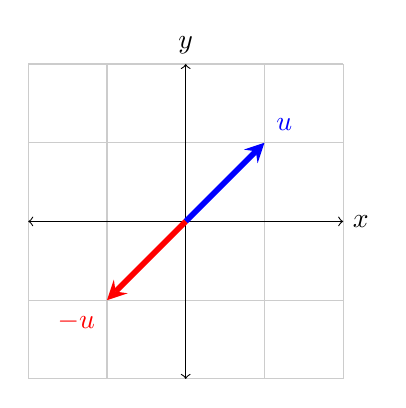
\begin{tikzpicture}
  \draw[thin,gray!40] (-2,-2) grid (2,2);
  \draw[<->] (-2,0)--(2,0) node[right]{$x$};
  \draw[<->] (0,-2)--(0,2) node[above]{$y$};
  \draw[line width=2pt,blue,-stealth](0,0)--(1,1)
        node[anchor=south west]{$\boldsymbol{u}$};
  \draw[line width=2pt,red,-stealth](0,0)--(-1,-1)
        node[anchor=north east]{$\boldsymbol{-u}$};
\end{tikzpicture}
\end{center}
\caption{\label{fig:vectors} Text size inside figure should be as big as
  caption's text.}
\end{figure}
%% %---------------------------


Here's a typical reference to a floating figure:
Figure~\ref{fig:vectors}. Floats should usually be placed where latex
wants then. Figure\ref{fig:vectors} is centered, and has a caption
that instructs you to make sure that the size of the text within the
figures that you use is as big as (or bigger than) the size of the
text in the caption of the figures. Please do. Really.

In our case, we've explicitly drawn the figure inlined in latex, to
allow this tex file to cleanly compile. But usually, your figures will
reside in some file.pdf, and you'd include them in your document
with, say, \textbackslash{}includegraphics.

Lists are sometimes quite handy. If you want to itemize things, feel
free:

\begin{description}
  
\item[fread] a function that reads from a \texttt{stream} into the
  array \texttt{ptr} at most \texttt{nobj} objects of size
  \texttt{size}, returning returns the number of objects read.

\item[Fred] a person's name, e.g., there once was a dude named Fred
  who separated usenix.sty from this file to allow for easy
  inclusion.
\end{description}

\noindent
The noindent at the start of this paragraph in its tex version makes
it clear that it's a continuation of the preceding paragraph, as
opposed to a new paragraph in its own right.
